%! TEX root = **/010-main.tex
% vim: spell spelllang=en:

\section{Machine learning methods}%
\label{sec:ml-methods}

% For  each  method  you  should  describe  how  you  adjusted  parameters  for  the algorithm and
% how did you perform an evaluation of the method.  You have to report also the performance of the model
% on the validation dataset. In addition,for each method you should describe and discus some particular issues:

%! TEX root = **/010-main.tex
% vim: spell spelllang=en:

\subsection{Na\"ive Bayes}%
\label{sub:naive-bayes}

\newcommand{\sresults}[2]{
\begin{table}[H]
\centering
\begin{tabular}{lc}
Confusion matrix on test set: & \( \begin{bmatrix} #1 \end{bmatrix} \) \\
    \addlinespace[0.5em]
    Accuracy on test set: & #2
\end{tabular}
\end{table}
}

\newcommand{\fresults}[3]{
\begin{table}[H]
\centering
\begin{tabular}{lc}
Confusion matrix on test set: & \( \begin{bmatrix} #1 \end{bmatrix} \) \\
    \addlinespace[0.5em]
    Accuracy on test set: & #2 \\
    F1 score on test set: & #3
\end{tabular}
\end{table}
}

% Think about hypothesis of independence of variables.  Do you have enough number of elements to obtain reliable probabilities?
% Keep that information for the discussion section.


Na\"ive Bayes works on the assumption of independence between variables in the dataset. First of all we checked weather or not 
this is a reasonable assumption in our dataset. To do so we calculated the correlation matrix, the farther apart the correlations 
are from 0 the more dependence there is between variables.

% Add correlation Matrix image

Despite seeing some strong correlations between pairs of variables, for most pairs these values are much closer to 0 than expected. 
Therefore it isn't that far-fetched to assume independence between variables.

There are several types of Na\"ive Bayes algorithms:
\begin{itemize}[topsep=0pt]
    \item Gaussian NB: Used when feature space is quantitative
    \item Bernoulli NB: Used when feature space is Binary
    \item Multinomial NB: Used when feature space is discrete counts
\end{itemize}

Our data is mostly numerical quantitative variables variables, therefore Gaussian Na\"ive Bayes will be applied from here on.

\subsection{Normalization}

First of all we executed the algorithm without performing any extra preprocessing of the data and obtained
relative poor results.

\fresults{208 & 200 \\ 3 & 189}{0.661}{0.65}

One of the problems we had when performing Na\"ive Bayes is that most of our data are continuous variables
which don't exactly follow a normal distribution. When using Gaussian Na\"ive Bayes will treat out data 
as if they followed such distribution. Therefore we tried different normalization techniques to make our
data more Gaussian-like

\subsection{Standardization}

After standardizing out data, std=1, mean=0. We executed the algorithm again and found better results:

\fresults{287 & 121 \\ 2 & 190}{0.795}{0.755}

\subsection{Power Transforms}

Power transforms is a preprocessing algorithm that simply explained aims to make our data more Gaussian-like. We executed Gaussian Na\"ive Bayes and found by far the best results:

\fresults{357 & 51 \\ 19 & 173}{0.883}{0.831}

We find it quite surprising to see how different normalization techniques yield such 
different final accuracy and f1-score results. We decided to continue forward with the Power 
Transformed data because it had by far the best results.

\subsection{Parameter tuning}

Na\"ive Bayes doesn't have many hyperparameters, in fact we will only analyse \texttt{var\_smoothing} which determines the amount Laplace smoothing applied.

\begin{figure}[H]
    \centering
    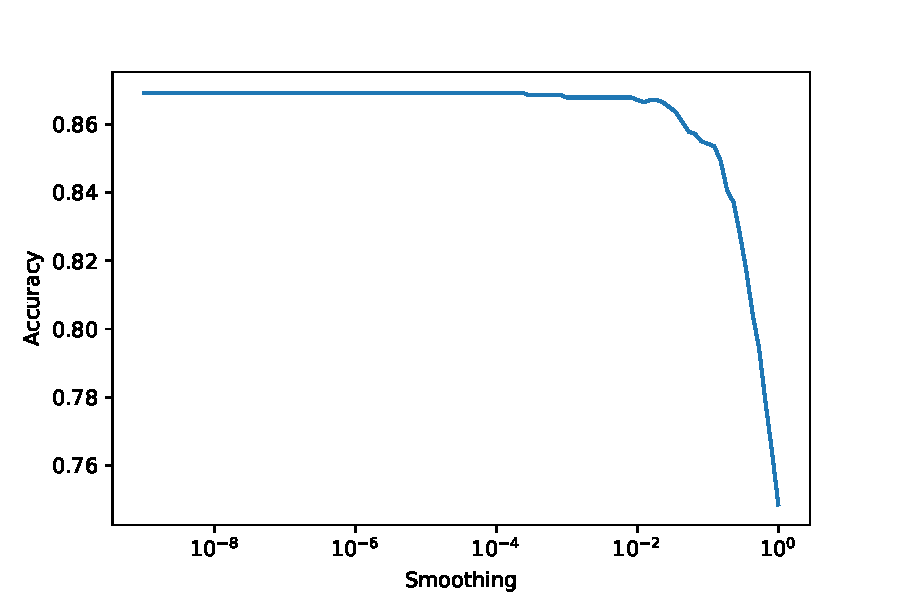
\includegraphics{figures/naive_bayes_smoothing_cv.pdf}
    \caption{Na\"ive Bayes smoothing}%
    \label{fig:naive_bayes_smoothing_cv}
\end{figure}

Looking at the image we can see that the accuracy barely changes when the \texttt{var\_smoothing} is in the range $[10^{-9}, 10^{-2}]$. Therefore its better to leave the default $10^{-9}$.

%! TEX root = **/010-main.tex
% vim: spell spelllang=en:

\subsection{K-NN}%
\label{sub:knn}
\begin{figure}[H]
    \centering
    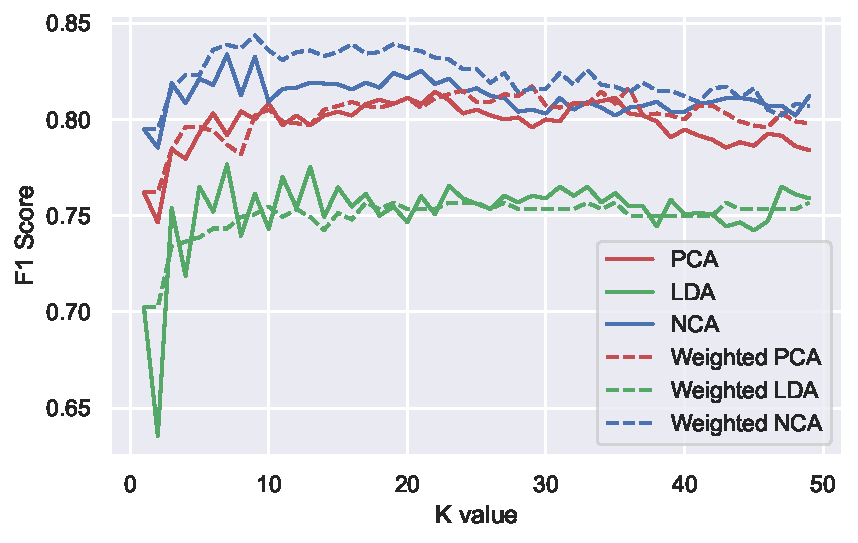
\includegraphics{knn2}
    \caption{weighted and unweighted knn with PCA, LDA and NCA}%
    \label{fig:knn_pca_lda_nca}
\end{figure}
% Description of procedure followed for choosing the best k-parameter. Show  a  graph  with  varying  k.  
% Have  you  adjusted  other  parameters  as distance measure? 
% Have you considered removal of irrelevant features if accuracy  is  poor  compared  with  other  approaches?   
% (remember  that  k-nn  is  sensible  to  irrelevant  features  when  computing  distance  to  closest examples

%! TEX root = **/010-main.tex
% vim: spell spelllang=en:

\subsection{Decision Trees}%
\label{sub:decision-trees}
We decided that in order to find the ideal depth of the decision tree, we had to try a range of values and pick the best performing one.

We tried all values between 1 and 50 and we found out that the best performing depth was around 5. 

\begin{figure}[H]
    \centering
    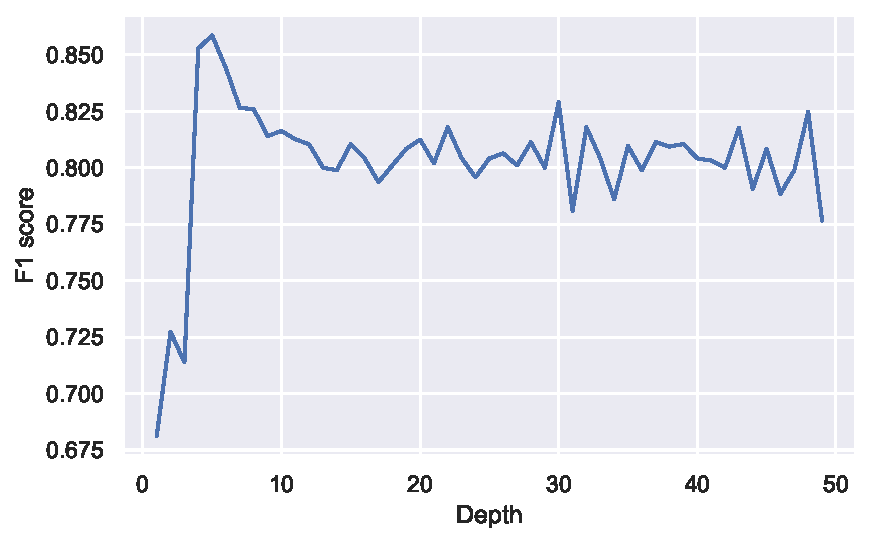
\includegraphics{decision_trees}
    \caption{decision trees accuracy depending on the depth.}%
    \label{fig:decision_trees_acc}
\end{figure}

\begin{figure}[H]
    \centering
    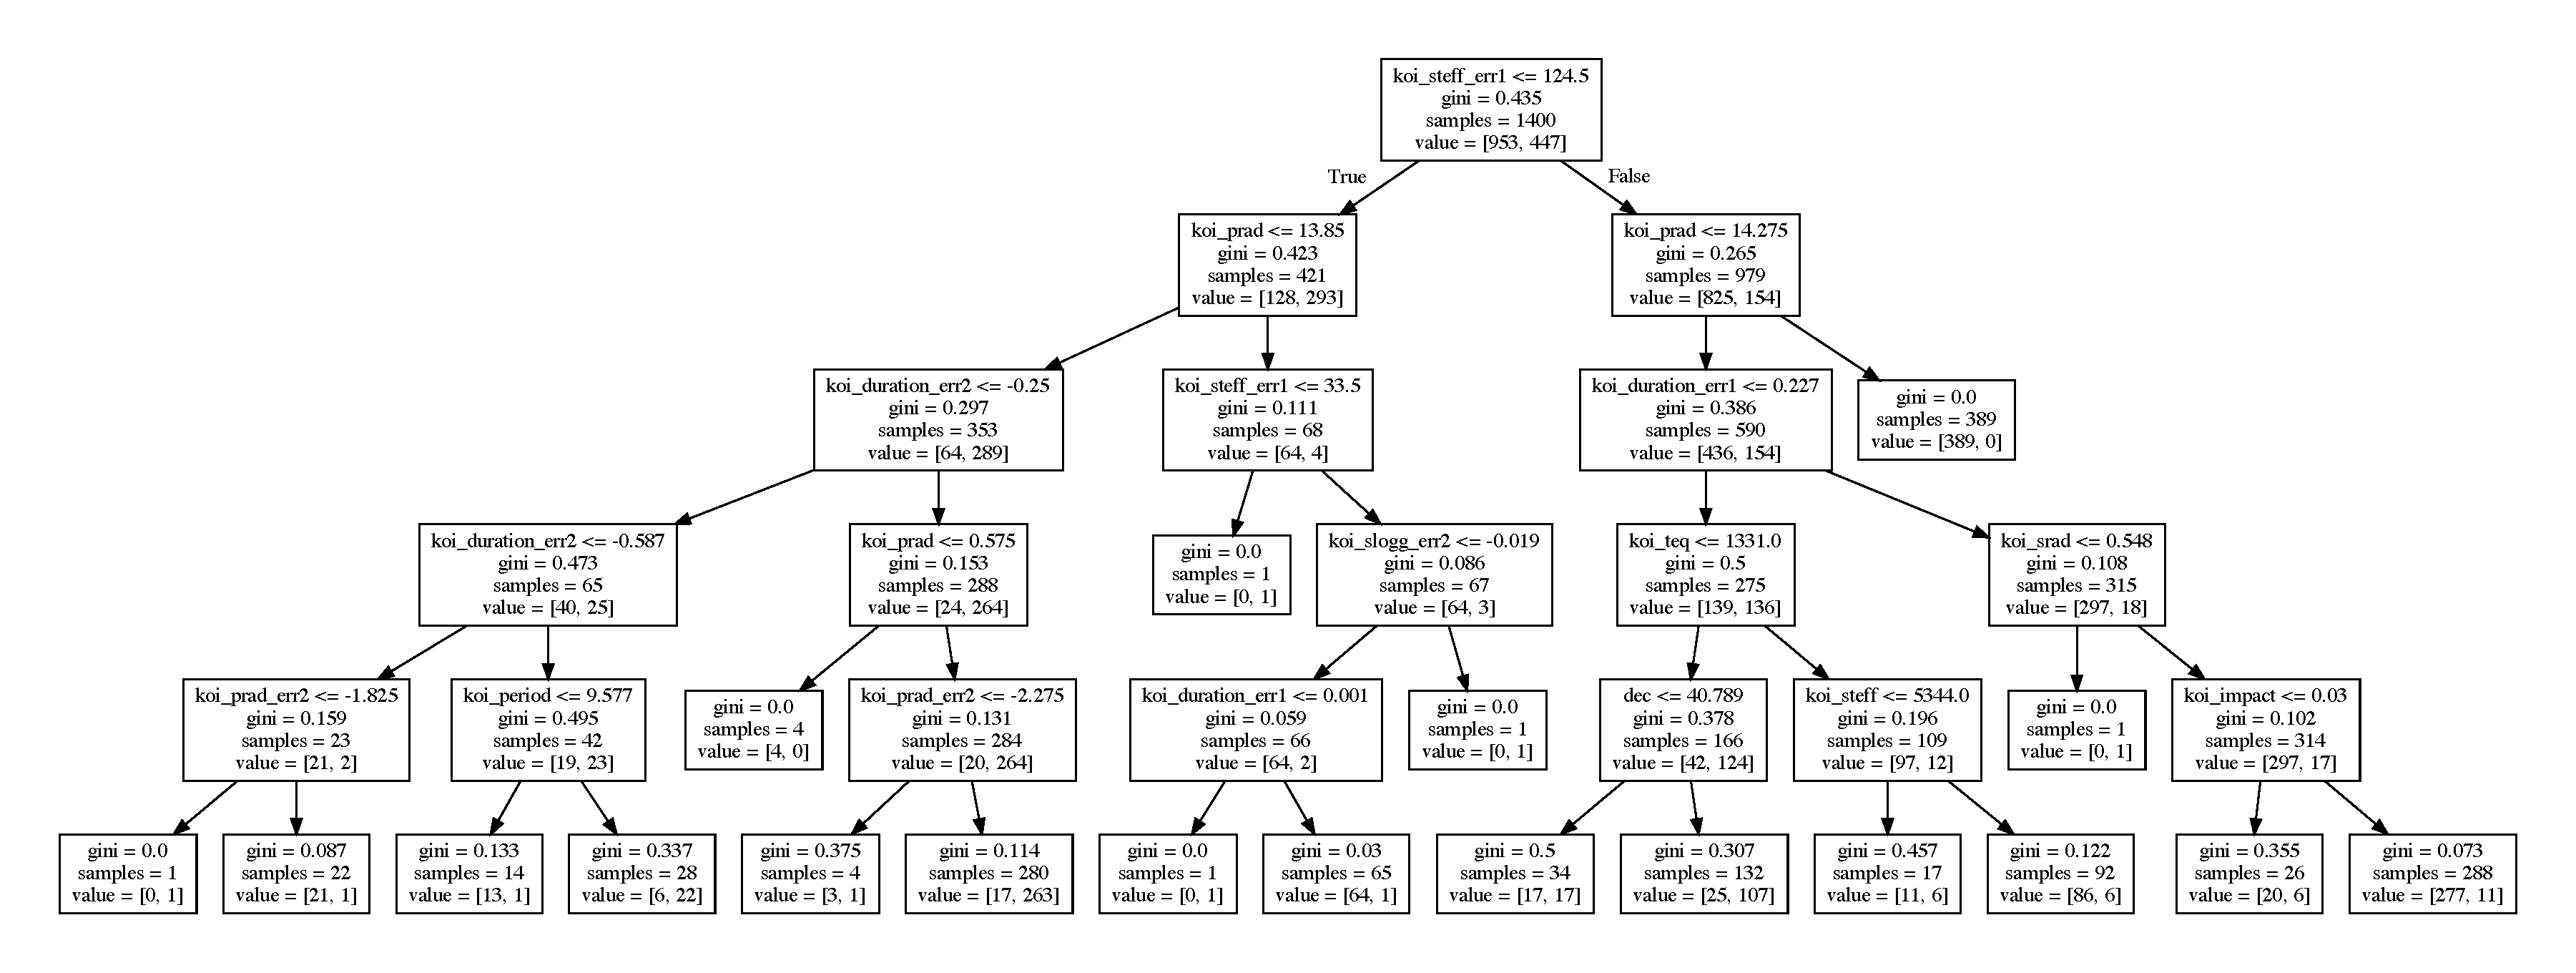
\includegraphics[width=\textwidth]{decision_tree}
    \caption{decision trees accuracy depending on the depth.}%
    \label{fig:decision_trees}
\end{figure}

% Discussion of choice of parameters used. Try to interpret the obtained DT using some examples of the validation set. 
% Show some of the most relevant rules.  Discuss how + and – examples are mixed in leaves in order to
% estimate the reliability of the tree.
%! TEX root = **/010-main.tex
% vim: spell spelllang=en:

\subsection{Support vector Machines}%
\label{sub:svm}

% discuss  choice  of  kernel  and  parameters used.  Did you run any method to speed the building of the model?
% Report number of supports of the selected machine and try to interpret why the kernel  selected  and
% parameters  selected  for  the  final  run  give  you  the best results for your dataset.
% Try also to inspect main supports of your machine.

We tried various kernels and performed a grid search for the best parameters for each one. When doing the search, we
performed a 5-fold cross validation since with 10 folds it took too much time and the results where fairly similar.
We also tried to reduce the number of features to 12 (from the 25 we selected in \cref{sub:feature_removal}) to reduce
execution time but the results where significantly worse (around 0.15 less accuracy).

In our case, the best results where obtained with a linear kernel with $C=10^5$.
In the following sections we show in detail the best results obtained with every kernel and a plot of the parameter search.

\subsection{Linear SVM}

With default parameters we obtained the following results:

\newcommand{\results}[7]{
\begin{table}[H]
\centering
\begin{tabular}{lc}
\toprule
\multicolumn{2}{c}{Best results (#3)} \\
\midrule
Confusion matrix on test set: & \( \begin{bmatrix} #1 \end{bmatrix} \) \\
    \addlinespace[0.5em]
    Accuracy on test set: & #2 \\
    F1 on test set: & #3 \\
    \addlinespace[1em]
    Number of supports: & #5 (#6 of them have slacks) \\
    Proportion of supports: & #7 \\
    \bottomrule
\end{tabular}
\end{table}
}


\fresults{387 & 21 \\ 54 & 138}{0.875}{0.7863}

By tuning the $C$ parameter as show in \cref{fig:svm_linear_C_cv} we managed to get much better results.

\begin{figure}[H]
    \centering
    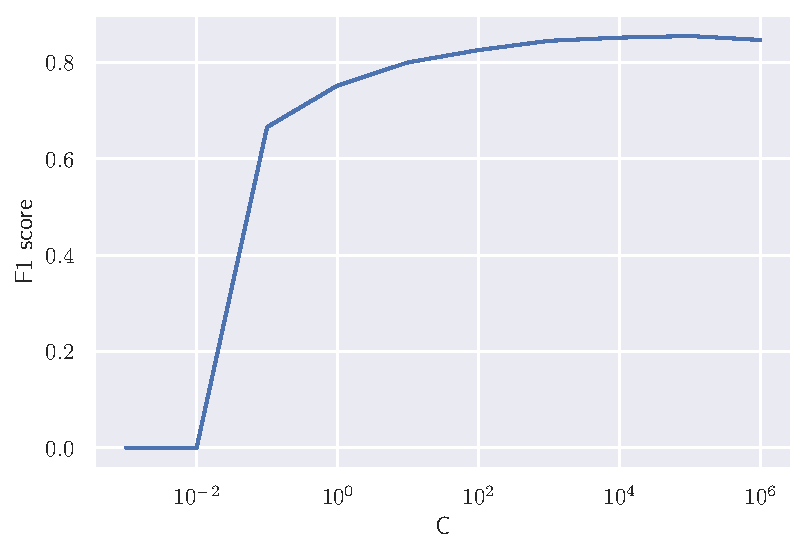
\includegraphics{svm_linear_C_cv}
    \caption{linear SVM C parameter search}%
    \label{fig:svm_linear_C_cv}
\end{figure}



\results{383 & 25 \\ 26 & 166}{0.915}{0.8668}{$C=10^5$}{288}{269}{0.2057}

We can see that the number of false positives in our confusion matrix halved with respect to the
default value. We achieved an accuracy of 0.915 and the proportion of supports is only $20\%$

\subsection{Polynomial SVM}

\results{380 & 28 \\ 28 & 164}{0.9067}{0.8542}{$C=10^4$}{332}{283}{0.2371}

\begin{figure}[H]
    \centering
    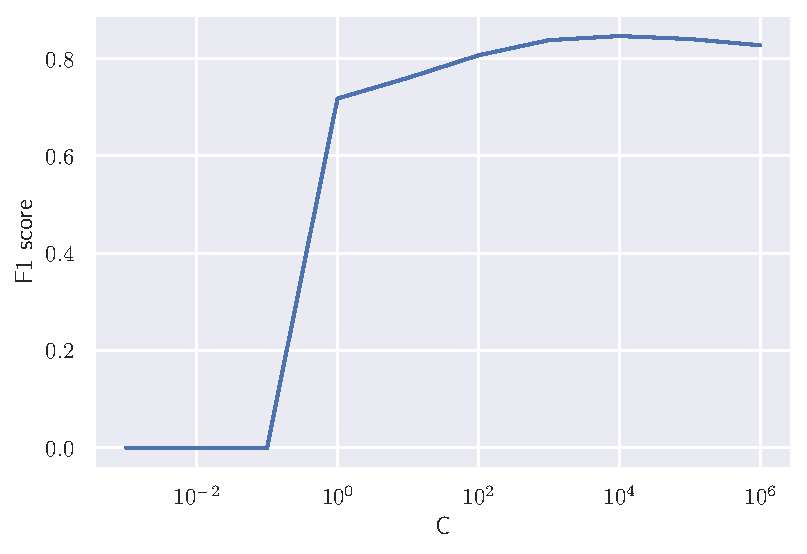
\includegraphics{svm_poly_C_cv}
    \caption{2nd degree polynomial SVM C parameter search}%
    \label{fig:svm_poly_C_cv}
\end{figure}

\results{381 & 27 \\ 30 & 162}{0.905}{0.8503}{$C=10^3$}{356}{317}{0.2543}

\begin{figure}[H]
    \centering
    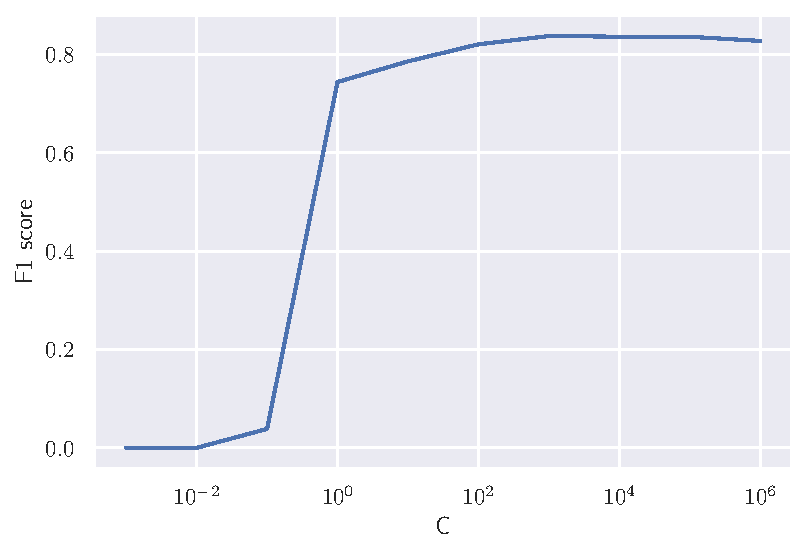
\includegraphics{svm_poly3_C_cv}
    \caption{3rd degree polynomial SVM C parameter search}%
    \label{fig:svm_poly3_C_cv}
\end{figure}

We obtained better results with the second degree polynomial although they both have similar accuracy. The linear
kernel outperformed both of them and had less support vectors.

\pagebreak
\subsection{RBF SVM}

With RBF we obtain better accuracy than with polynomial kernels but still not as good as with the linear kernel.

\results{381 & 27 \\ 28 & 164}{0.9083}{0.8564}{$C=10^6, gamma=0.001$}{330}{302}{0.2357}

\begin{figure}[H]
    \centering
    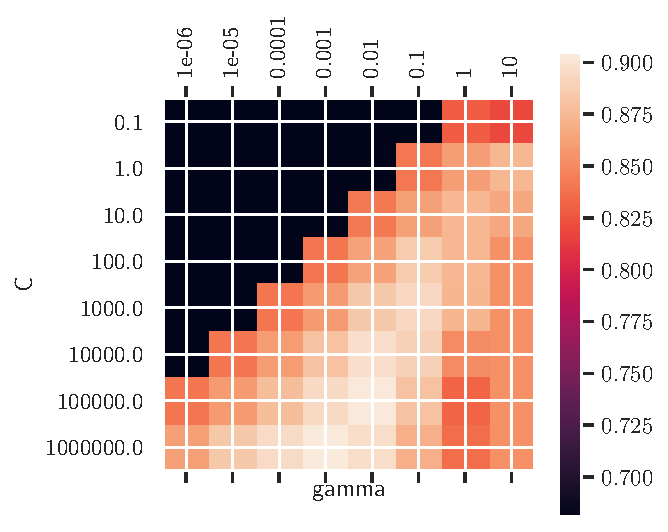
\includegraphics{svm_rbf_C_cv}
    \caption{RBF SVM C parameter search}%
    \label{fig:svm_rbf_C_cv}
\end{figure}

%! TEX root = **/010-main.tex
% vim: spell spelllang=en:

\subsection{Meta-learning algorithms}%
\label{sub:meta}

\subsubsection{Performance Majority Voting}

Majority voting uses several of the algorithms already commented in this project. Therefore we will use those algorithms with the best combination of preprocessing and hyperparameters we already found.

\begin{table}[H]
\centering
\caption{Majority voting results}
\begin{tabular}{lr}
\toprule
Method & Accuracy \\
\midrule
Na\"ive Bayes & 0.884 \\
K-NN & 0.857 \\
Decision Tree & 0.877 \\
\addlinespace[0.5em]
Majority voting & 0.914 \\
Majority voting (weighted)  & 0.914 \\
\bottomrule
\end{tabular}
\end{table}


With hard voting:
\fresults{ 375 &  33 \\ 20 & 172 }{ 0.9117 }{ 0.8622 }

\noindent
With weighted voting (2 1 2):
\fresults{ 373 &  35 \\ 19 & 173 }{ 0.9100 }{ 0.8492 }

There is no benefit to weighting the votes since all 3 methods offer very similar accuracy.

\pagebreak
\subsubsection{Bagging}

\begin{figure}[H]
\centering
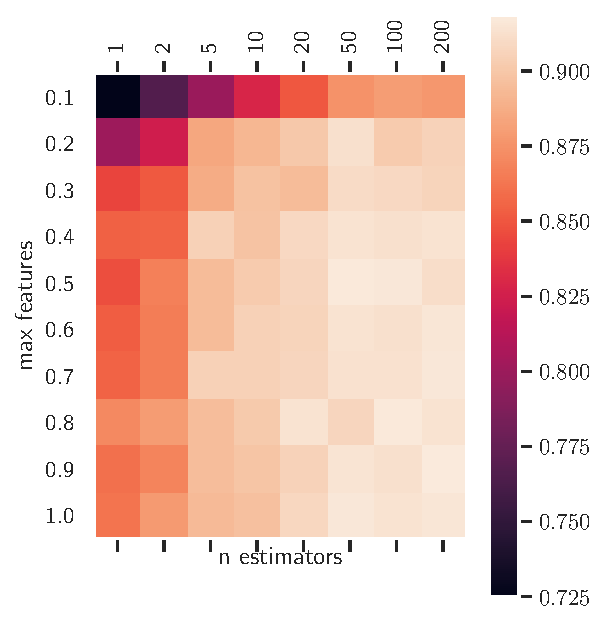
\includegraphics{bagging}
\caption{Bagging parameter search}%
\label{fig:bagging}
\end{figure}

The best results where obtained with: $\texttt{n\_est} = 200, \texttt{max\_features} = 0.9$. Nonetheless, as we
can see in \cref{fig:bagging} results with $\texttt{n\_est} \geq 50, \texttt{max\_features} \geq 0.3$ are pretty
similar.

\fresults{ 388 &  20 \\ 24  & 168 }{0.9267}{0.8825}

\begin{verbatim}
\end{verbatim}

\pagebreak
\subsubsection{RandomForest}

Random Forest is an algorithm based in the combination of multiple decision trees. It has many hyperparameters among which we decided to optimize the 6 following: \texttt{bootstrap}, \texttt{max\_features}, \texttt{max\_features}, \texttt{min\_samples\_leaf}, \texttt{min\_samples\_split}, \texttt{n\_estimators}. At the beginning we wanted to have a pool of
many values per parameter. However the time of computation was too high and we ended up doing a 5-fold with 2-3 values per parameter.

\begin{table}[H]
\centering
\caption{RandomForest best parameters}
\begin{tabular}{lr}
\toprule
Parameter & Value \\
\midrule
\texttt{bootstrap} & True \\
\texttt{max\_depth} & 150 \\
\texttt{max\_features} & 10 \\
\texttt{min\_samples\_leaf} & 5 \\
\texttt{min\_samples\_split} & 5 \\
\texttt{n\_estimators} & 500 \\
\bottomrule
\end{tabular}
\end{table}

\fresults{ 384 &  24 \\ 21 & 171 }{0.925}{0.883}
\pagebreak
\subsubsection{Adaboost}

The final algorithm we implemented is Ada boosting. The base implementation of this algorithms works with decision trees as it's classifier. This type of boosting basically consists on performing different executions of the classifier but changing the weights. The algorithm has two additional hyperparameters \texttt{n\_estimators} and \texttt{learning\_rate}.

After that we fined tuned the parameters and we found that the best combination is \texttt{n\_estimators} = 60 and \texttt{learning\_rate} = 0.5

\begin{figure}[H]
\centering
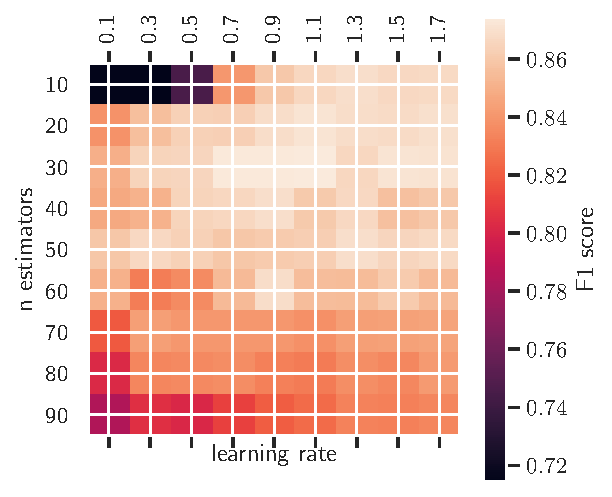
\includegraphics{boosting}
\caption{AdaBoost parameter search}%
\label{fig:boosting}
\end{figure}

When executing Adaboost with the best parameters found we obtain the following results:

\fresults{ 383 &  25 \\ 21 & 171 }{0.923}{0.881}


% Performance  Majority  Voting,  Bagging, RandomForest  and  Adaboost.   Explain  parameters  selected  for  each  algorithm

